\section{Example: TPC-H Q10}

We consider TPC-H Q10 over the four relations:
$N=\textsf{nation}$, $C=\textsf{customer}$, $O=\textsf{orders}$, $L=\textsf{lineitem}$.
Let $U_R$ denote the (effective) batch size of updates to relation $R$ in one round
(predicate-conditioned, after applying query predicates).


%%%%%%%%%%%%%%%%%%%%%%%%%%%%%%%%%%%%%%%%%%%%%%%%%%%%%%%%%%%%%%%%%%%%%%%%%%%%%%
% vo1: orderkey -> custkey -> nationkey
%%%%%%%%%%%%%%%%%%%%%%%%%%%%%%%%%%%%%%%%%%%%%%%%%%%%%%%%%%%%%%%%%%%%%%%%%%%%%%
\subsection{vo1: $\texttt{orderkey} \rightarrow \texttt{custkey} \rightarrow \texttt{nationkey}$}

\begin{figure}[ht]
\centering
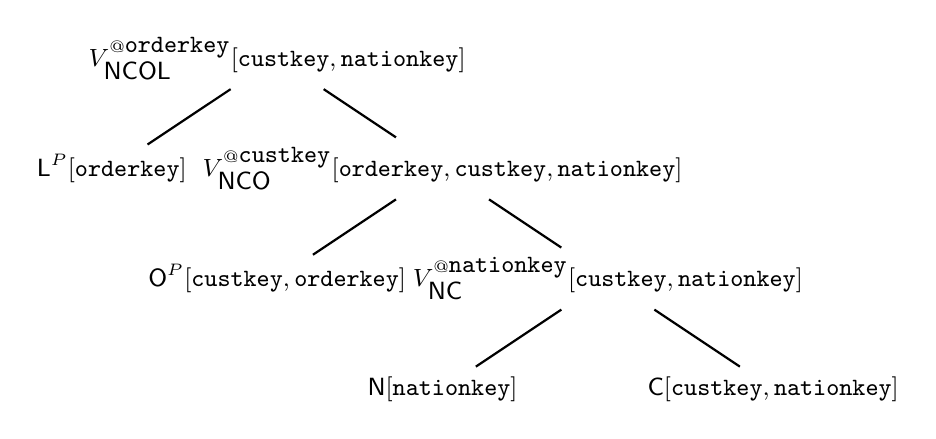
\begin{tikzpicture}[
  level distance=14mm,
  sibling distance=42mm,
  every node/.style={font=\small, align=center},
  edge from parent/.style={draw, thick}
]
\node (Vo)
{$V^{@\texttt{orderkey}}_{\textsf{NCOL}}[\texttt{custkey},\texttt{nationkey}]$}
  child { node (L)
    {$\textsf{L}^{P}[\texttt{orderkey}]$}
  }
  child { node (Vc)
    {$V^{@\texttt{custkey}}_{\textsf{NCO}}[\texttt{orderkey},\texttt{custkey},\texttt{nationkey}]$}
      child { node (O)
        {$\textsf{O}^{P}[\texttt{custkey},\texttt{orderkey}]$}
      }
      child { node (Vn)
        {$V^{@\texttt{nationkey}}_{\textsf{NC}}[\texttt{custkey},\texttt{nationkey}]$}
          child { node (N)
            {$\textsf{N}[\texttt{nationkey}]$}
          }
          child { node (C)
            {$\textsf{C}[\texttt{custkey},\texttt{nationkey}]$}
          }
      }
  };
\end{tikzpicture}
\caption{View tree vo1. The root $\texttt{orderkey}$-node is an aggregation node.}
\label{fig:vo1}
\end{figure}

\paragraph{Symbolic cost.}
Aggregation at root; N and C traverse 3 hops to reach it.
\begin{align*}
S_L &= \delta^{\mathrm{join}}_L + \delta^{\mathrm{agg}}_L,
\quad \delta^{\mathrm{join}}_L = U_L \cdot \deg_{V_{NCO}}(*|\texttt{okey}),\\[4pt]
S_O &= \delta_O + \delta^{\mathrm{join}}_O + \delta^{\mathrm{agg}}_O,
\quad \delta_O = U_O \cdot \deg_{V_{NC}}(*|\texttt{ckey}),\;
\delta^{\mathrm{join}}_O = \delta_O \cdot \deg_{L^P}(*|\texttt{okey}),\\[4pt]
S_C &= \delta^{(1)}_C + \delta^{(2)}_C + \delta^{\mathrm{join}}_C + \delta^{\mathrm{agg}}_C,\\
&\quad \delta^{(1)}_C = U_C \cdot \deg_N(*|\texttt{nkey}),\;
\delta^{(2)}_C = \delta^{(1)}_C \cdot \deg_{O^P}(*|\texttt{ckey}),\;
\delta^{\mathrm{join}}_C = \delta^{(2)}_C \cdot \deg_{L^P}(*|\texttt{okey}),\\[4pt]
S_N &= \delta^{(1)}_N + \delta^{(2)}_N + \delta^{\mathrm{join}}_N + \delta^{\mathrm{agg}}_N,\\
&\quad \delta^{(1)}_N = U_N \cdot \deg_C(*|\texttt{nkey}),\;
\delta^{(2)}_N = \delta^{(1)}_N \cdot \deg_{O^P}(*|\texttt{ckey}),\;
\delta^{\mathrm{join}}_N = \delta^{(2)}_N \cdot \deg_{L^P}(*|\texttt{okey}).
\end{align*}
All $\delta^{\mathrm{agg}} = \min(\delta^{\mathrm{join}}, |\mathrm{Dom}(\texttt{okey})|)$.
\[
\boxed{\mathrm{Score}_{\mathrm{vo1}} = S_N + S_C + S_O + S_L}
\]

\paragraph{Statistics (TPC-H SF=1).}
We compare statistics with and without query predicates
($O^P$: \texttt{o\_orderdate} $\in$ [1993-10-01, 1994-01-01);
$L^P$: \texttt{l\_returnflag} = 'R').

\smallskip
\noindent\textbf{Update batch sizes} (per 10000-tuple global batch, distributed by table size).
\begin{center}
\begin{tabular}{lrrl}
\toprule
& With Predicates & No Predicates & Note \\
\midrule
$U_N$ & 0 or 1 & 0 or 1 & (scenario-dependent) \\
$U_C$ & 196 & 196 & no predicate on $C$ \\
$U_O$ & 75 & 1961 & selectivity 3.8\% \\
$U_L$ & 1933 & 7844 & selectivity 24.6\% \\
\bottomrule
\end{tabular}
\end{center}

\paragraph{Grounded scores.}

\smallskip
\noindent\textbf{Static scenario ($U_N = 0$).}
\begin{center}
\begin{tabular}{lrr}
\toprule
& With Predicates & No Predicates \\
\midrule
$S_N$ & 0 & 0 \\
$S_C$ & 570 & 17843 \\
$S_O$ & 374 & 17647 \\
$S_L$ & 294 & 15687 \\
\midrule
\textbf{Total} & \textbf{1238} & \textbf{51178} \\
\bottomrule
\end{tabular}
\end{center}

\smallskip
\noindent\textbf{Dynamic scenario ($U_N = 1$).}
Nation updates are expensive (3-hop path to root).
\begin{center}
\begin{tabular}{lrr}
\toprule
& With Predicates & No Predicates \\
\midrule
$S_N$ & 17460 & 546097 \\
$S_C$ & 570 & 17843 \\
$S_O$ & 374 & 17647 \\
$S_L$ & 294 & 15687 \\
\midrule
\textbf{Total} & \textbf{18698} & \textbf{597275} \\
\bottomrule
\end{tabular}
\end{center}

%%%%%%%%%%%%%%%%%%%%%%%%%%%%%%%%%%%%%%%%%%%%%%%%%%%%%%%%%%%%%%%%%%%%%%%%%%%%%%
% vo2: orderkey -> nationkey -> custkey
%%%%%%%%%%%%%%%%%%%%%%%%%%%%%%%%%%%%%%%%%%%%%%%%%%%%%%%%%%%%%%%%%%%%%%%%%%%%%%
\subsection{vo2: $\texttt{orderkey} \rightarrow \texttt{nationkey} \rightarrow \texttt{custkey}$}

\begin{figure}[ht]
\centering
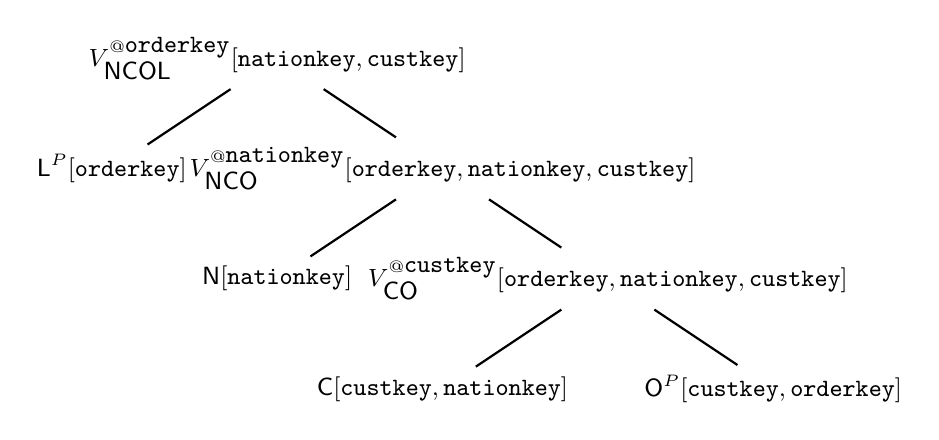
\begin{tikzpicture}[
  level distance=14mm,
  sibling distance=42mm,
  every node/.style={font=\small, align=center},
  edge from parent/.style={draw, thick}
]
\node (Vo)
{$V^{@\texttt{orderkey}}_{\textsf{NCOL}}[\texttt{nationkey},\texttt{custkey}]$}
  child { node (L)
    {$\textsf{L}^{P}[\texttt{orderkey}]$}
  }
  child { node (Vn)
    {$V^{@\texttt{nationkey}}_{\textsf{NCO}}[\texttt{orderkey},\texttt{nationkey},\texttt{custkey}]$}
      child { node (N)
        {$\textsf{N}[\texttt{nationkey}]$}
      }
      child { node (Vc)
        {$V^{@\texttt{custkey}}_{\textsf{CO}}[\texttt{orderkey},\texttt{nationkey},\texttt{custkey}]$}
          child { node (C)
            {$\textsf{C}[\texttt{custkey},\texttt{nationkey}]$}
          }
          child { node (O)
            {$\textsf{O}^{P}[\texttt{custkey},\texttt{orderkey}]$}
          }
      }
  };
\end{tikzpicture}
\caption{View tree vo2. The root $\texttt{orderkey}$-node is an aggregation node.}
\label{fig:vo2}
\end{figure}

\paragraph{Symbolic cost.}
Aggregation at root; N is at depth 2, C and O at depth 3.
\begin{align*}
S_L &= \delta^{\mathrm{join}}_L + \delta^{\mathrm{agg}}_L,
\quad \delta^{\mathrm{join}}_L = U_L \cdot \deg_{V_{NCO}}(*|\texttt{okey}),\\[4pt]
S_N &= \delta_N + \delta^{\mathrm{join}}_N + \delta^{\mathrm{agg}}_N,
\quad \delta_N = U_N \cdot \deg_{V_{CO}}(*|\texttt{nkey}),\;
\delta^{\mathrm{join}}_N = \delta_N \cdot \deg_{L^P}(*|\texttt{okey}),\\[4pt]
S_C &= \delta^{(1)}_C + \delta^{(2)}_C + \delta^{\mathrm{join}}_C + \delta^{\mathrm{agg}}_C,\\
&\quad \delta^{(1)}_C = U_C \cdot \deg_{O^P}(*|\texttt{ckey}),\;
\delta^{(2)}_C = \delta^{(1)}_C \cdot \deg_N(*|\texttt{nkey}),\;
\delta^{\mathrm{join}}_C = \delta^{(2)}_C \cdot \deg_{L^P}(*|\texttt{okey}),\\[4pt]
S_O &= \delta^{(1)}_O + \delta^{(2)}_O + \delta^{\mathrm{join}}_O + \delta^{\mathrm{agg}}_O,\\
&\quad \delta^{(1)}_O = U_O \cdot \deg_C(*|\texttt{ckey}),\;
\delta^{(2)}_O = \delta^{(1)}_O \cdot \deg_N(*|\texttt{nkey}),\;
\delta^{\mathrm{join}}_O = \delta^{(2)}_O \cdot \deg_{L^P}(*|\texttt{okey}).
\end{align*}
All $\delta^{\mathrm{agg}} = \min(\delta^{\mathrm{join}}, |\mathrm{Dom}(\texttt{okey})|)$.
\[
\boxed{\mathrm{Score}_{\mathrm{vo2}} = S_N + S_C + S_O + S_L}
\]

\paragraph{Grounded scores.}

\smallskip
\noindent\textbf{Static scenario ($U_N = 0$).}
\begin{center}
\begin{tabular}{lrr}
\toprule
& With Predicates & No Predicates \\
\midrule
$S_N$ & 0 & 0 \\
$S_C$ & 449 & 19608 \\
$S_O$ & 449 & 19608 \\
$S_L$ & 294 & 15687 \\
\midrule
\textbf{Total} & \textbf{1192} & \textbf{54903} \\
\bottomrule
\end{tabular}
\end{center}

\smallskip
\noindent\textbf{Dynamic scenario ($U_N = 1$).}
Nation updates are cheaper than vo1 (2-hop vs.\ 3-hop path).
\begin{center}
\begin{tabular}{lrr}
\toprule
& With Predicates & No Predicates \\
\midrule
$S_N$ & 11459 & 540097 \\
$S_C$ & 449 & 19608 \\
$S_O$ & 449 & 19608 \\
$S_L$ & 294 & 15687 \\
\midrule
\textbf{Total} & \textbf{12651} & \textbf{595000} \\
\bottomrule
\end{tabular}
\end{center}

%%%%%%%%%%%%%%%%%%%%%%%%%%%%%%%%%%%%%%%%%%%%%%%%%%%%%%%%%%%%%%%%%%%%%%%%%%%%%%
% vo3: nationkey -> custkey -> orderkey
%%%%%%%%%%%%%%%%%%%%%%%%%%%%%%%%%%%%%%%%%%%%%%%%%%%%%%%%%%%%%%%%%%%%%%%%%%%%%%
\subsection{vo3: $\texttt{nationkey} \rightarrow \texttt{custkey} \rightarrow \texttt{orderkey}$}

\begin{figure}[ht]
\centering
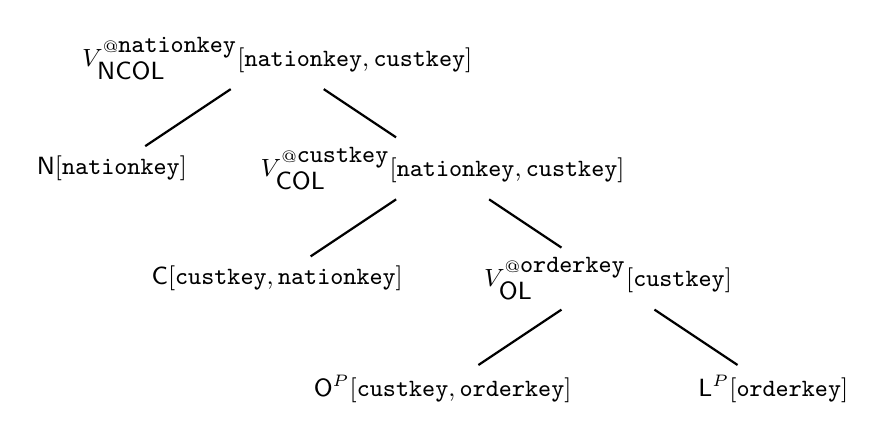
\begin{tikzpicture}[
  level distance=14mm,
  sibling distance=42mm,
  every node/.style={font=\small, align=center},
  edge from parent/.style={draw, thick}
]
\node (Vn)
{$V^{@\texttt{nationkey}}_{\textsf{NCOL}}[\texttt{nationkey},\texttt{custkey}]$}
  child { node (N)
    {$\textsf{N}[\texttt{nationkey}]$}
  }
  child { node (Vc)
    {$V^{@\texttt{custkey}}_{\textsf{COL}}[\texttt{nationkey},\texttt{custkey}]$}
      child { node (C)
        {$\textsf{C}[\texttt{custkey},\texttt{nationkey}]$}
      }
      child { node (Vo)
        {$V^{@\texttt{orderkey}}_{\textsf{OL}}[\texttt{custkey}]$}
          child { node (O)
            {$\textsf{O}^{P}[\texttt{custkey},\texttt{orderkey}]$}
          }
          child { node (L)
            {$\textsf{L}^{P}[\texttt{orderkey}]$}
          }
      }
  };
\end{tikzpicture}
\caption{View tree vo3. The $\texttt{orderkey}$-node is an aggregation node with output key \texttt{custkey}.}
\label{fig:vo3}
\end{figure}

\paragraph{Symbolic cost.}
\begin{align*}
S_N &= U_N \cdot \deg_{V_{COL}}(*|\texttt{nkey}), \\[4pt]
S_C &= U_C \cdot \deg_{V_{OL}}(*|\texttt{ckey}) \cdot (1 + \deg_N(*|\texttt{nkey})), \\[4pt]
S_O &= (\delta^{\mathrm{join}}_O + \delta^{\mathrm{agg}}_O) \cdot (1 + \deg_C(*|\texttt{ckey}) \cdot (1 + \deg_N(*|\texttt{nkey}))),
\\
&\qquad \text{where } \delta^{\mathrm{join}}_O = U_O \cdot \deg_{L^P}(*|\texttt{okey}),\;
\delta^{\mathrm{agg}}_O = \min(\delta^{\mathrm{join}}_O,\, |\mathrm{Dom}(\texttt{ckey})|), \\[4pt]
S_L &= (\delta^{\mathrm{join}}_L + \delta^{\mathrm{agg}}_L) \cdot (1 + \deg_C(*|\texttt{ckey}) \cdot (1 + \deg_N(*|\texttt{nkey}))),
\\
&\qquad \text{where } \delta^{\mathrm{join}}_L = U_L \cdot \deg_{O^P}(*|\texttt{okey}),\;
\delta^{\mathrm{agg}}_L = \min(\delta^{\mathrm{join}}_L,\, |\mathrm{Dom}(\texttt{ckey})|).
\end{align*}
\[
\boxed{\mathrm{Score}_{\mathrm{vo3}} = S_N + S_C + S_O + S_L}
\]

\paragraph{Grounded scores.}

\smallskip
\noindent\textbf{Static scenario ($U_N = 0$).}
\begin{center}
\begin{tabular}{lrr}
\toprule
& With Predicates & No Predicates \\
\midrule
$S_N$ & 0 & 0 \\
$S_C$ & 99 & 261 \\
$S_O$ & 900 & 47061 \\
$S_L$ & 881 & 47061 \\
\midrule
\textbf{Total} & \textbf{1880} & \textbf{94383} \\
\bottomrule
\end{tabular}
\end{center}

\smallskip
\noindent\textbf{Dynamic scenario ($U_N = 1$).}
\begin{center}
\begin{tabular}{lrr}
\toprule
& With Predicates & No Predicates \\
\midrule
$S_N$ & 1519 & 6000 \\
$S_C$ & 99 & 261 \\
$S_O$ & 900 & 47061 \\
$S_L$ & 881 & 47061 \\
\midrule
\textbf{Total} & \textbf{3398} & \textbf{100383} \\
\bottomrule
\end{tabular}
\end{center}

\paragraph{Observations.}
\begin{itemize}
\item Without predicates, the cost is $\sim$50$\times$ higher due to larger update batch sizes and higher fanouts.
\item A single nation update adds significant cost due to the large degree $\deg_{V_{COL}}(*|\texttt{nkey})$
(each nation matches $\sim$1500--6000 customers).
\end{itemize}

%%%%%%%%%%%%%%%%%%%%%%%%%%%%%%%%%%%%%%%%%%%%%%%%%%%%%%%%%%%%%%%%%%%%%%%%%%%%%%
% vo4: nationkey -> orderkey -> custkey
%%%%%%%%%%%%%%%%%%%%%%%%%%%%%%%%%%%%%%%%%%%%%%%%%%%%%%%%%%%%%%%%%%%%%%%%%%%%%%
\subsection{vo4: $\texttt{nationkey} \rightarrow \texttt{orderkey} \rightarrow \texttt{custkey}$}

\begin{figure}[ht]
\centering
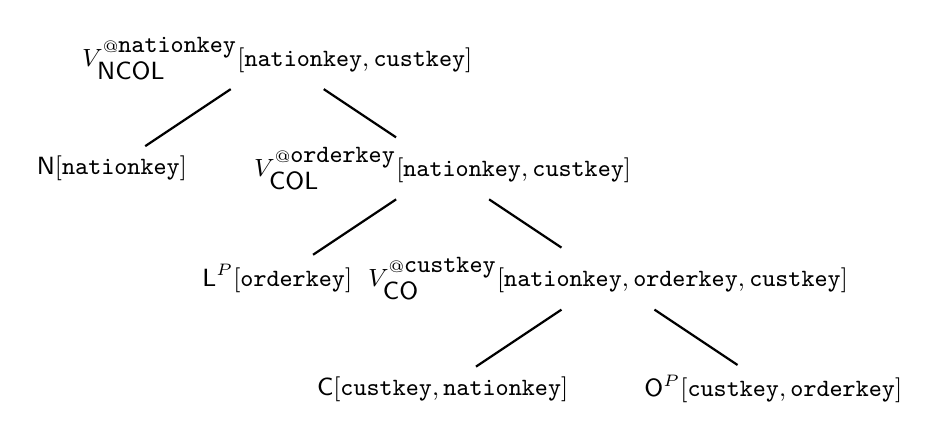
\begin{tikzpicture}[
  level distance=14mm,
  sibling distance=42mm,
  every node/.style={font=\small, align=center},
  edge from parent/.style={draw, thick}
]
\node (Vn)
{$V^{@\texttt{nationkey}}_{\textsf{NCOL}}[\texttt{nationkey},\texttt{custkey}]$}
  child { node (N)
    {$\textsf{N}[\texttt{nationkey}]$}
  }
  child { node (Vo)
    {$V^{@\texttt{orderkey}}_{\textsf{COL}}[\texttt{nationkey},\texttt{custkey}]$}
      child { node (L)
        {$\textsf{L}^{P}[\texttt{orderkey}]$}
      }
      child { node (Vc)
        {$V^{@\texttt{custkey}}_{\textsf{CO}}[\texttt{nationkey},\texttt{orderkey},\texttt{custkey}]$}
          child { node (C)
            {$\textsf{C}[\texttt{custkey},\texttt{nationkey}]$}
          }
          child { node (O)
            {$\textsf{O}^{P}[\texttt{custkey},\texttt{orderkey}]$}
          }
      }
  };
\end{tikzpicture}
\caption{View tree vo4. The $\texttt{orderkey}$-node is an aggregation node with output key \texttt{custkey}.}
\label{fig:vo4}
\end{figure}

\paragraph{Symbolic cost.}
\begin{align*}
S_N &= U_N \cdot \deg_{V_{COL}}(*|\texttt{nkey}), \\[4pt]
S_L &= (\delta^{\mathrm{join}}_L + \delta^{\mathrm{agg}}_L) \cdot (1 + \deg_N(*|\texttt{nkey})),
\quad \delta^{\mathrm{join}}_L = U_L \cdot \deg_{V_{CO}}(*|\texttt{okey}),\\[4pt]
S_C &= \delta_C + (\delta^{\mathrm{join}}_C + \delta^{\mathrm{agg}}_C) \cdot (1 + \deg_N(*|\texttt{nkey})),
\quad \delta_C = U_C \cdot \deg_{O^P}(*|\texttt{ckey}),\;
\delta^{\mathrm{join}}_C = \delta_C \cdot \deg_{L^P}(*|\texttt{okey}),\\[4pt]
S_O &= \delta_O + (\delta^{\mathrm{join}}_O + \delta^{\mathrm{agg}}_O) \cdot (1 + \deg_N(*|\texttt{nkey})),
\quad \delta_O = U_O \cdot \deg_C(*|\texttt{ckey}),\;
\delta^{\mathrm{join}}_O = \delta_O \cdot \deg_{L^P}(*|\texttt{okey}).
\end{align*}
All $\delta^{\mathrm{agg}} = \min(\delta^{\mathrm{join}}, |\mathrm{Dom}(\texttt{ckey})|)$.
\[
\boxed{\mathrm{Score}_{\mathrm{vo4}} = S_N + S_C + S_O + S_L}
\]

\paragraph{Grounded scores.}

\smallskip
\noindent\textbf{Static scenario ($U_N = 0$).}
\begin{center}
\begin{tabular}{lrr}
\toprule
& With Predicates & No Predicates \\
\midrule
$S_N$ & 0 & 0 \\
$S_C$ & 674 & 33334 \\
$S_O$ & 674 & 33334 \\
$S_L$ & 587 & 31374 \\
\midrule
\textbf{Total} & \textbf{1936} & \textbf{98042} \\
\bottomrule
\end{tabular}
\end{center}

\smallskip
\noindent\textbf{Dynamic scenario ($U_N = 1$).}
\begin{center}
\begin{tabular}{lrr}
\toprule
& With Predicates & No Predicates \\
\midrule
$S_N$ & 1519 & 6000 \\
$S_C$ & 674 & 33334 \\
$S_O$ & 674 & 33334 \\
$S_L$ & 587 & 31374 \\
\midrule
\textbf{Total} & \textbf{3454} & \textbf{104042} \\
\bottomrule
\end{tabular}
\end{center}

%%%%%%%%%%%%%%%%%%%%%%%%%%%%%%%%%%%%%%%%%%%%%%%%%%%%%%%%%%%%%%%%%%%%%%%%%%%%%%
% vo5: bushy (custkey root; children: nationkey and orderkey)
%%%%%%%%%%%%%%%%%%%%%%%%%%%%%%%%%%%%%%%%%%%%%%%%%%%%%%%%%%%%%%%%%%%%%%%%%%%%%%
\subsection{vo5: bushy (root \texttt{custkey}; children \texttt{nationkey}, \texttt{orderkey})}

\begin{figure}[ht]
\centering
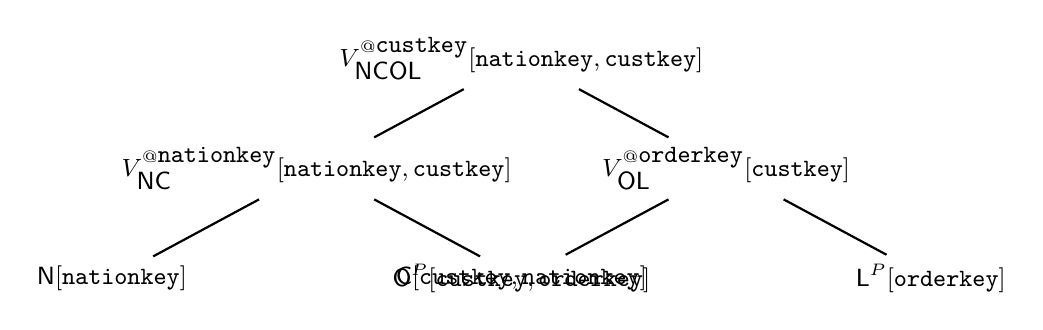
\begin{tikzpicture}[
  level distance=14mm,
  sibling distance=52mm,
  every node/.style={font=\small, align=center},
  edge from parent/.style={draw, thick}
]
\node (Vc)
{$V^{@\texttt{custkey}}_{\textsf{NCOL}}[\texttt{nationkey},\texttt{custkey}]$}
  child { node (Vn)
    {$V^{@\texttt{nationkey}}_{\textsf{NC}}[\texttt{nationkey},\texttt{custkey}]$}
      child { node (N)
        {$\textsf{N}[\texttt{nationkey}]$}
      }
      child { node (C)
        {$\textsf{C}[\texttt{custkey},\texttt{nationkey}]$}
      }
  }
  child { node (Vo)
    {$V^{@\texttt{orderkey}}_{\textsf{OL}}[\texttt{custkey}]$}
      child { node (O)
        {$\textsf{O}^{P}[\texttt{custkey},\texttt{orderkey}]$}
      }
      child { node (L)
        {$\textsf{L}^{P}[\texttt{orderkey}]$}
      }
  };
\end{tikzpicture}
\caption{View tree vo5 (bushy). The $\texttt{orderkey}$-node is an aggregation node.}
\label{fig:vo5}
\end{figure}

\paragraph{Symbolic cost.}
Bushy tree: N/C branch and O/L branch meet at the root.
\begin{align*}
S_C &= \delta_C \cdot (1 + \deg_{V_{OL}}(*|\texttt{ckey})),
\quad \delta_C = U_C \cdot \deg_N(*|\texttt{nkey}), \\[4pt]
S_N &= \delta_N \cdot (1 + \deg_{V_{OL}}(*|\texttt{ckey})),
\quad \delta_N = U_N \cdot \deg_C(*|\texttt{nkey}), \\[4pt]
S_O &= (\delta^{\mathrm{join}}_O + \delta^{\mathrm{agg}}_O) \cdot (1 + \deg_{V_{NC}}(*|\texttt{ckey})),
\quad \delta^{\mathrm{join}}_O = U_O \cdot \deg_{L^P}(*|\texttt{okey}),\\[4pt]
S_L &= (\delta^{\mathrm{join}}_L + \delta^{\mathrm{agg}}_L) \cdot (1 + \deg_{V_{NC}}(*|\texttt{ckey})),
\quad \delta^{\mathrm{join}}_L = U_L \cdot \deg_{O^P}(*|\texttt{okey}).
\end{align*}
$\delta^{\mathrm{agg}} = \min(\delta^{\mathrm{join}}, |\mathrm{Dom}(\texttt{ckey})|)$.
\[
\boxed{\mathrm{Score}_{\mathrm{vo5}} = S_N + S_C + S_O + S_L}
\]

\paragraph{Grounded scores.}

\smallskip
\noindent\textbf{Static scenario ($U_N = 0$).}
\begin{center}
\begin{tabular}{lrr}
\toprule
& With Predicates & No Predicates \\
\midrule
$S_N$ & 0 & 0 \\
$S_C$ & 246 & 327 \\
$S_O$ & 600 & 31374 \\
$S_L$ & 587 & 31374 \\
\midrule
\textbf{Total} & \textbf{1433} & \textbf{63074} \\
\bottomrule
\end{tabular}
\end{center}

\smallskip
\noindent\textbf{Dynamic scenario ($U_N = 1$).}
Nation updates are cheap (only 2-hop, no aggregation traversal).
\begin{center}
\begin{tabular}{lrr}
\toprule
& With Predicates & No Predicates \\
\midrule
$S_N$ & 7518 & 10000 \\
$S_C$ & 246 & 327 \\
$S_O$ & 600 & 31374 \\
$S_L$ & 587 & 31374 \\
\midrule
\textbf{Total} & \textbf{8951} & \textbf{73074} \\
\bottomrule
\end{tabular}
\end{center}

%%%%%%%%%%%%%%%%%%%%%%%%%%%%%%%%%%%%%%%%%%%%%%%%%%%%%%%%%%%%%%%%%%%%%%%%%%%%%%
% Summary
%%%%%%%%%%%%%%%%%%%%%%%%%%%%%%%%%%%%%%%%%%%%%%%%%%%%%%%%%%%%%%%%%%%%%%%%%%%%%%
\subsection{Summary and Rankings}

\paragraph{Cost comparison.}
\begin{center}
\begin{tabular}{lrrrr}
\toprule
& \multicolumn{2}{c}{With Predicates} & \multicolumn{2}{c}{No Predicates} \\
\cmidrule(lr){2-3} \cmidrule(lr){4-5}
VO & Static & Dynamic & Static & Dynamic \\
\midrule
vo1 & 1238 & 18698 & 51178 & 597275 \\
vo2 & 1192 & 12651 & 54903 & 595000 \\
vo3 & 1880 & 3398 & 94383 & 100383 \\
vo4 & 1936 & 3454 & 98042 & 104042 \\
vo5 & 1433 & 8951 & 63074 & 73074 \\
\bottomrule
\end{tabular}
\end{center}

\paragraph{Rankings by scenario.}

\smallskip
\noindent\textbf{Static scenario ($U_N = 0$): dimension tables not updated.}
\begin{center}
\begin{tabular}{clrclr}
\toprule
\multicolumn{3}{c}{With Predicates} & \multicolumn{3}{c}{No Predicates} \\
\cmidrule(lr){1-3} \cmidrule(lr){4-6}
Rank & VO & Score & Rank & VO & Score \\
\midrule
1 & vo2 & 1192 & 1 & vo1 & 51178 \\
2 & vo1 & 1238 & 2 & vo2 & 54903 \\
3 & vo5 & 1433 & 3 & vo5 & 63074 \\
4 & vo3 & 1880 & 4 & vo3 & 94383 \\
5 & vo4 & 1936 & 5 & vo4 & 98042 \\
\bottomrule
\end{tabular}
\end{center}

\smallskip
\noindent\textbf{Dynamic scenario ($U_N = 1$): dimension tables updated.}
\begin{center}
\begin{tabular}{clrclr}
\toprule
\multicolumn{3}{c}{With Predicates} & \multicolumn{3}{c}{No Predicates} \\
\cmidrule(lr){1-3} \cmidrule(lr){4-6}
Rank & VO & Score & Rank & VO & Score \\
\midrule
1 & vo3 & 3398 & 1 & vo5 & 73074 \\
2 & vo4 & 3454 & 2 & vo3 & 100383 \\
3 & vo5 & 8951 & 3 & vo4 & 104042 \\
4 & vo2 & 12651 & 4 & vo2 & 595000 \\
5 & vo1 & 18698 & 5 & vo1 & 597275 \\
\bottomrule
\end{tabular}
\end{center}

\paragraph{Key observations.}
\begin{itemize}
\item The optimal variable order depends critically on whether the nation table is updated:
  \begin{itemize}
  \item \textbf{Static nation:} vo1 and vo2 are best---placing the aggregation node at the root minimizes the path length for high-frequency O/L updates.
  \item \textbf{Dynamic nation:} vo3 and vo4 are best---placing nation near the root (depth 1) keeps $S_N$ small.
  \end{itemize}
\item vo1 and vo2 place nation at depth 3 and 2, respectively. A single nation update propagates through multiple joins, causing $S_N$ to explode (e.g., 18k vs.\ 3k for vo3 with predicates).
\item vo5 (bushy) provides a robust compromise: ranked 3rd in static scenarios and 1st--3rd in dynamic scenarios.
\item Predicates reduce total cost by $\sim$50$\times$ due to smaller effective batch sizes and lower join fanouts.
\end{itemize}
